\lecture{26}{4. December 2025}{Plane strain transformation \& strain rosettes}

\subsection{Plane Strain}
The general state of strain at a point in a body is represented by a combination of three components of normal strain, $\epsilon_x$, $\epsilon_y$, $\epsilon_z$ and three components of shear strain $\gamma_{xy}$, $\gamma_{xz}$, $\gamma_{yz}$.
The normal strains cause a change in the volume of the element, and the shear strains cause a change in shape.


\subsection{General Equations of Plane-Strain Transformation}
The plane-strain analysis it is important to establish strain transformation equations that can be used to determine the components of normal and shear strain at a point $\epsilon_{x'}$, $\epsilon_{y'}$, $\gamma_{x'y'}$, provided the components $\epsilon_x$, $\epsilon_y$, $\gamma_{xy}$ are known (as depicted on \Cref{fig:f14_26}.

\begin{figure} [ht]
  \centering
  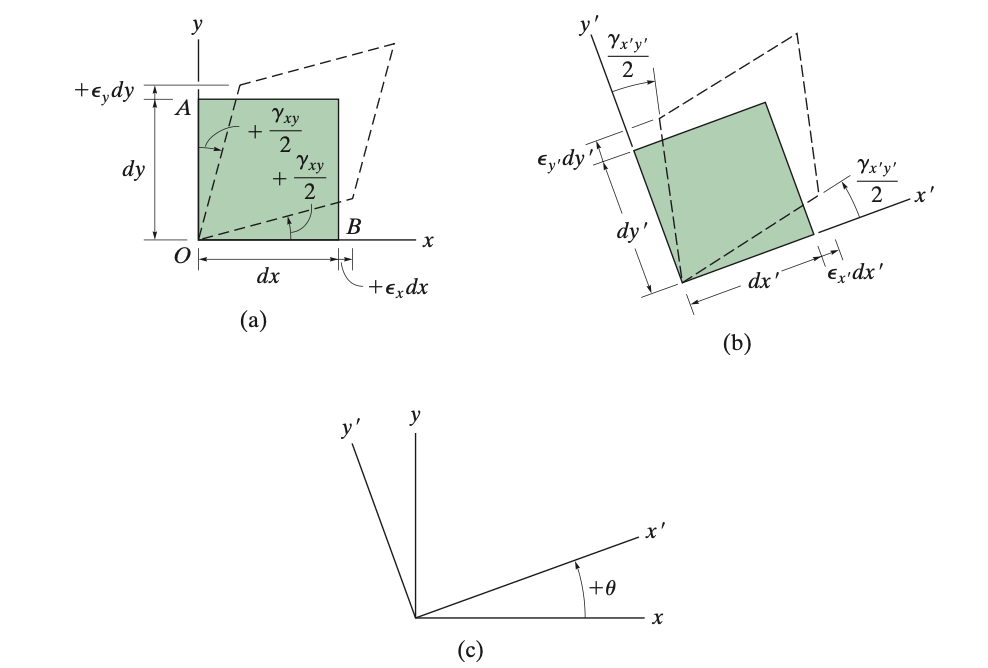
\includegraphics[width=0.5\linewidth]{./figures/f14_26.png}
  \caption{Plane-strain transformation.}
  \label{fig:f14_26}
\end{figure}

\paragraph{Sign Convention}
The normal strains $\epsilon_x$ and $\epsilon_y$ in \Cref{fig:f14_26}a are positive if they cause elongation along the $x$ and $y$ axes and the shear strain $\gamma_{xy}$ is positive if the interior angle $AOB$ becomes smaller than \ang{90}.

Finally, if the angle between the $x$ and $x'$ axes is $\theta$ then $\theta$ will be positive if it follows the curl of the right-hand fingers, i.e. counterclockwise. 

\paragraph{Normal and Shear Strains}
We have the general results:
\begin{align*}
  \epsilon_{x'} &= \frac{\epsilon_x + \epsilon_y}{2} + \frac{\epsilon_x - \epsilon_y}{2} \cos 2\theta + \frac{\gamma_{xy}}{2} \sin 2\theta \\
  \epsilon_{y'} &= \frac{\epsilon_x + \epsilon_y}{2} - \frac{\epsilon_x - \epsilon_y}{2} \cos 2\theta - \frac{\gamma_{xy}}{2} \sin 2\theta \\
  \frac{\gamma_{x'y'}}{2} &= - \left( \frac{\epsilon_x - \epsilon_y}{2} \right) \sin 2\theta + \frac{\gamma_{xy}}{2} \cos 2\theta
.\end{align*}

\paragraph{Principal Strains}
Like stress, an element can be oriented at a point so that the element's deformation is caused only by normal strains, with no shear strain. 
When this occurs, the normal strains are referred to as \textit{principal strains}, and if the material is isotropic, the axes along which these strains occur will coincide with the axes of principal stress.

The direction of the $x'$ axis and the two values of the principal strains $\epsilon_1$ and $\epsilon_2$ are determined from:
\begin{align*}
  \tan 2\theta_p &= \frac{\gamma_{xy}}{\epsilon_x - \epsilon_y} \\
  \epsilon_{1,2} &= \frac{\epsilon_x + \epsilon_y}{2} \pm \sqrt{\left( \frac{\epsilon_x - \epsilon_y}{2} \right)^2 + \left( \frac{\gamma_{xy}}{2} \right)^2}
.\end{align*}

\paragraph{Maximum In-Plane Shear Strain}
We also have that:
\begin{align*}
  \tan 2\theta_s &= - \left( \frac{\epsilon_x - \epsilon_y}{\gamma_{xy}} \right) \\
  \frac{\gamma_{\mathrm{max}, \mathrm{in-plane}}}{2} &= \sqrt{\left( \frac{\epsilon_x - \epsilon_y}{2} \right)^2 + \left( \frac{\gamma_{xy}}{2} \right)^2} \\
  \epsilon_{\mathrm{avg}} &= \frac{\epsilon_x + \epsilon_y}{2}
.\end{align*}

\subsection{Strain Rosettes}
The normal strain on the free surface of a body can be measured in a particular direction using an electrical resistance strain gauge.
Unfortunately, the shear strain cannot be measured directly with a strain gauge, so to obtain $\epsilon_x$, $\epsilon_y$, $\gamma_{xy}$, we must use a cluster of three strain gauges that are arranges in a pattern called a \textit{strain rosette}.

To show how this is done, we consider the general case of arranging the gauges at angles $\theta_a$, $\theta_b$, $\theta_c$ as shown in \Cref{fig:f14_40}a.
If the readings $\epsilon_a$, $\epsilon_b$, $\epsilon_c$ are obtained, we can determine the strain components using the normal strain transformation equations for each gauge resulting in
\begin{align*}
  \epsilon_a &= \epsilon_x \cos^2 \theta_a + \epsilon_y \sin^2 \theta_a + \gamma_{xy} \sin \theta_a \cos \theta_a \\
  \epsilon_b &= \epsilon_x \cos^2 \theta_b + \epsilon_y \sin^2 \theta_b + \gamma_{xy} \sin \theta_b \cos \theta_b \\
  \epsilon_c &= \epsilon_x \cos^2 \theta_c + \epsilon_y \sin^2 \theta_c + \gamma_{xy} \sin \theta_c \cos \theta_c
.\end{align*}

\begin{figure} [ht]
  \centering
  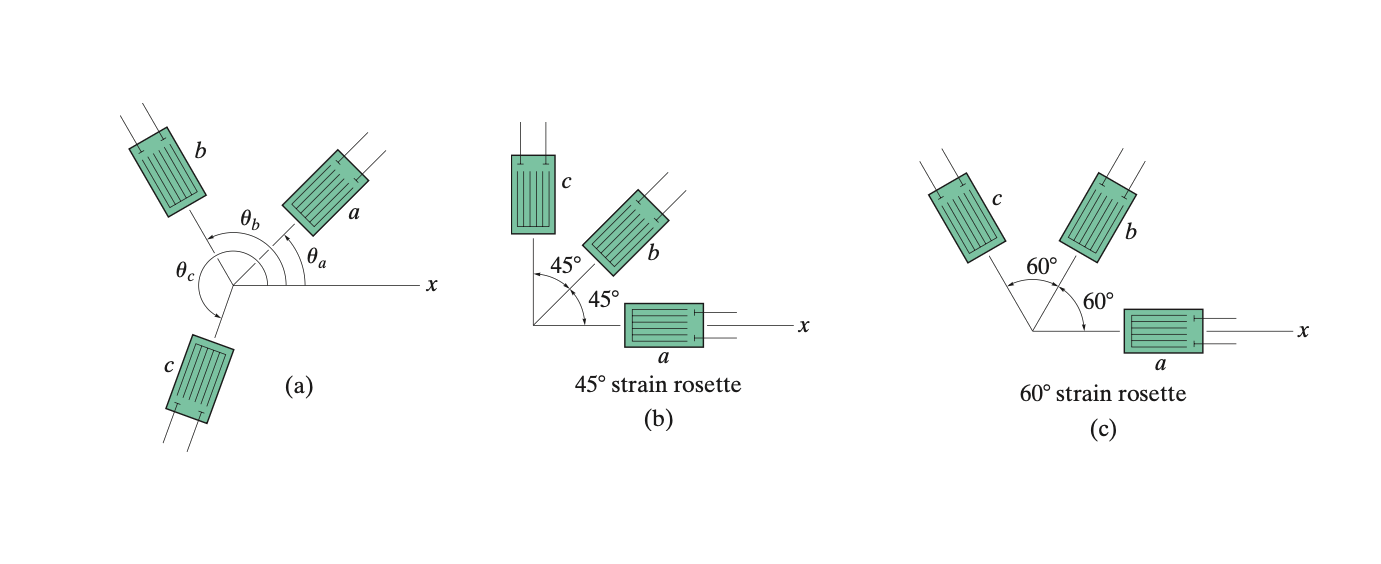
\includegraphics[width=\linewidth]{./figures/f14_40.png}
  \caption{Strain Rosettes.}
  \label{fig:f14_40}
\end{figure}  

\paragraph{\ang{45} Rosette}
In the case of the \ang{45} or ``rectangular'' strain rosette depicted on \Cref{fig:f14_40}b, $\theta_a = \ang{0}$, $\theta_b = \ang{45}$, $\theta_c = \ang{90} $, so
\begin{align*}
  \epsilon_x &= \epsilon_a \\
  \epsilon_y &= \epsilon_c \\
  \gamma_{xy} &= 2 \epsilon_b - \left( \epsilon_a + \epsilon_c \right)
.\end{align*}

\paragraph{\ang{60} Rosette}
For the \ang{60} strain rosette depicted on \Cref{fig:f14_40}c, $\theta_a = \ang{0}$, $\theta_b = \ang{60}$, $\theta_c = \ang{120}$.
Here
\begin{align*}
  \epsilon_x &= \epsilon_a \\
  \epsilon_y &= \frac{1}{3} \left( 2 \epsilon_b + 2\epsilon_c - \epsilon_a \right) \\
  \gamma_{xy} &= \frac{2}{\sqrt{3}} \left( \epsilon_b - \epsilon_c \right)
.\end{align*}
